\documentclass[10pt, handout]{beamer}

\usetheme[progressbar=frametitle]{metropolis}

\usepackage{appendixnumberbeamer}

\usepackage{booktabs}
\usepackage{blkarray}
%\usepackage{ccicons}
\usepackage{graphicx}
\usepackage{color}

\definecolor{UniBlue}{RGB}{7,82,154}
\definecolor{UniYellow}{RGB}{234,185,12}

%\setbeamercolor{title}{fg=UniBlue, bg = UniYellow}
%\setbeamercolor{frametitle}{fg=UniBlue, bg= UniYellow}
%\setbeamercolor{structure}{fg=UniBlue, bg= UniYellow}
%\setbeamercolor{progress bar}{fg=UniBlue, bg= UniYellow}
\usepackage{xspace}

\title{Multiscale Inference for Nonparametric Time Trends}
\date{\today}
\author{Marina Khismatullina \inst{1} \and Michael Vogt \inst{1}}
\institute{\inst{1} University of Bonn}
\setbeamertemplate{frame footer}{Multiscale Inference for Nonparametric Time Trends}
\metroset{block=fill}
% \titlegraphic{\hfill\includegraphics[height=1.5cm]{logo.pdf}}

\newcommand{\Prob}{\mathrm{P}}
\newcommand{\E}{\mathbb{E}}
\newcommand{\Var}{\mathrm{Var}}
\newcommand{\Cov}{\mathrm{Cov}}
\newcommand{\Corr}{\mathrm{Corr}}
\newcommand{\sgn}{\text{sgn}}
\newtheorem{prop}{Proposition}


\begin{document}

\maketitle

\begin{frame}{Table of contents}
  \setbeamertemplate{section in toc}[sections numbered]
  \tableofcontents[hideallsubsections]
\end{frame}

\section{Introduction}

\begin{frame}{Motivation}
	\begin{figure}
		\centering
		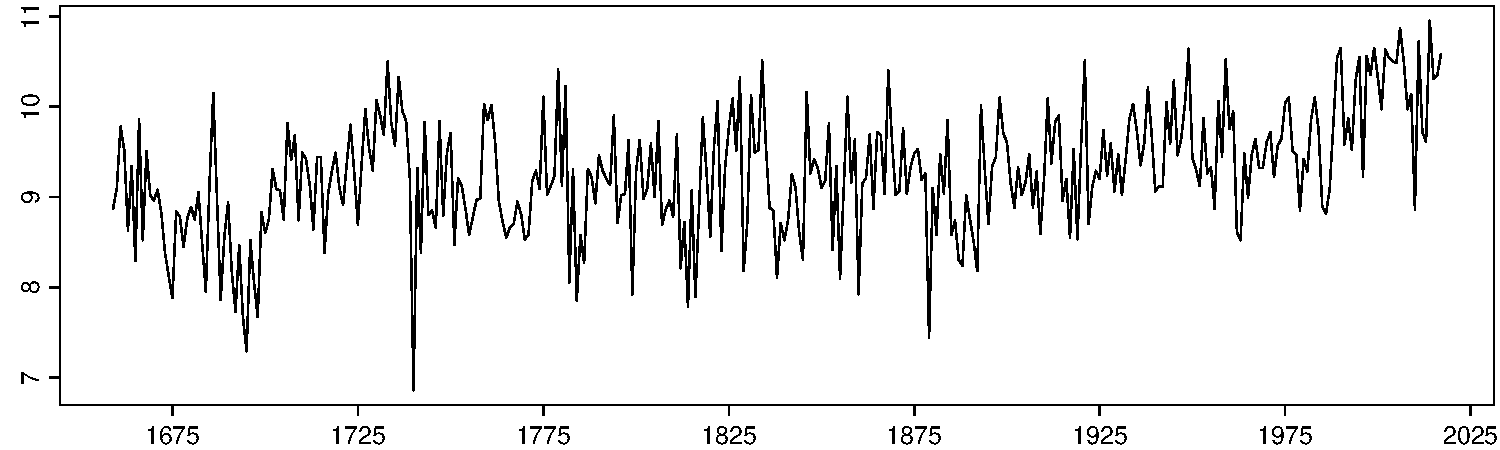
\includegraphics[width=\textwidth]{temperature_data.pdf}
		\caption{Yearly mean temperature in Central England from 1659 to 2017}
		\label{figure:temperature_data}
	\end{figure}\pause
	\begin{itemize}
		\item Does the observed time series have a trend at all?\pause
		\item If so, which are the time regions where there is a strong trend?\pause
		\item Is the trend decreasing or increasing in these regions?
	 \end{itemize}
\end{frame}

\begin{frame}{Idea}
    \begin{block}{Research question}
	Develop multiscale methods to test qualitative hypotheses about nonapametric time trends.\pause
	
	One time series is observed:
	\begin{itemize}
		\item Test the null hypothesis of the existence of a time trend.
		\item Identify time regions with upward or downward movement in the trend.
	\end{itemize}\pause
	Multiple time series are observed:
	\begin{itemize}
		\item  Detect which time trends are different and where.
	\end{itemize}
    \end{block}
\end{frame}

\section{Model}
\begin{frame}{Model}
We observe a single time series $\{Y_t: 1 \le t \le T \}$ of length $T$. The observations come from a following model:
\begin{equation*}\label{model1}
Y_t = m \Big( \frac{t}{T} \Big) + \varepsilon_t 
\end{equation*}\pause
\vspace{-6mm}
\begin{itemize}
\item $m$ is an unknown trend function on $[0,1]$;
\item $\{ \varepsilon_t: 1 \le t \le T \}$ is a zero-mean stationary error process.
\end{itemize}
\end{frame}

\begin{frame}{Literature}
	Multiscale approaches for independent data
	\begin{itemize}
		\item SiZer method (Chaudhuri and Marron, 1999, 2000)
		\item Testing monotonicity of the trend function (Hall and Heckman, 2000, D{\"u}mbgen and Spokoiny, 2001)
	\end{itemize}\pause
	Multiscale methods for dependent data
	\begin{itemize}
		\item Extensions to SiZer method (Park et al. 2004, 2009, Rondonotti et al. 2007)
	\end{itemize}
\end{frame}

\section{The multiscale method}
\subsection{Testing problem}
\begin{frame}{Testing}
Testing problem:
\begin{align*}
H_0:\quad &m = 0\\
H_1:\quad &m\not= 0
\end{align*}
\end{frame}

\subsection{Test statistic}
\begin{frame}{Test Statistic}
For a given location $u \in [0,1]$ and bandwidth $h$ we construct the kernel averages
\begin{equation*}
\widehat{\psi}_T(u,h) = \sum\limits_{t=1}^T w_{t,T}(u,h) Y_t, 
\end{equation*}\pause
\vspace{-3mm}
where 
\begin{align*}
w_{t,T}(u,h) &= \frac{\Lambda_{t,T}(u,h)}{ \{\sum\nolimits_{t=1}^T \Lambda_{t,T}^2(u,h)\}^{1/2} } ,\\
\Lambda_{t,T}(u,h) &= K\Big(\frac{t/T-u}{h}\Big) \Big[ S_{T,2}(u,h) - S_{T,1}(u,h) \Big(\frac{t/T-u}{h}\Big) \Big], \\
S_{T,\ell}(u,h) &= \frac{1}{Th} \sum\nolimits_{t=1}^T K\Big(\frac{t/T-u}{h}\Big) \Big(\frac{t/T-u}{h}\Big)^\ell
\end{align*}
for $\ell = 0,1,2$ and $K$ is a kernel function.
\end{frame}

\begin{frame}[label = frame_teststatistic]{Test Statistic}
Test statistic is defined as follows
\begin{equation*}
\widehat{\Psi}_T = \max_{(u,h) \in \mathcal{G}_T} \Big\{ \Big|\frac{\widehat{\psi}_T(u,h)}{\widehat{\sigma}}\Big| - \lambda(h) \Big\}, 
\end{equation*} \pause
where 
\begin{itemize}
\item $\widehat{\sigma}^2$ is an appropriate estimator of the long-run variance $\sigma^2$ (Hall and Van Keilegom (2003));
\item $\mathcal{G}_T$ is the set of points $(u,h)$ that are taken into consideration;
\item $\lambda(h) = \sqrt{2 \log \{ 1/(2h) \}}$ is an additive correction term (D{\"u}mbgen and Spokoiny (2001)). \hyperlink{frame_lambda}{\beamerbutton{Explanation}}
\end{itemize}
\end{frame}

\begin{frame}{Test procedure}
Gaussian version of the test statistic:
\begin{align*}
\Phi_T = \max_{(u,h) \in \mathcal{G}_T} \Big\{ \Big|\frac{\phi_T(u,h)}{\sigma}\Big| - \lambda(h) \Big\},
\end{align*} 
\vspace{-3mm}
where
\begin{itemize}
\item $\phi_T(u,h) = \sum\nolimits_{t=1}^T w_{t,T}(u,h) \, {\color<3>{mLightBrown}\sigma Z_t}$;
\item $Z_t$ are independent standard normal random variables;
\item $q_T(\alpha)$ is $(1 - \alpha)$ quantile of $\Phi_T$.
\end{itemize}\pause\pause
\begin{block}{Test procedure}
For a given significance level $\alpha \in (0,1)$, we reject $H_0$ if $\widehat{\Psi}_T > q_T(\alpha)$.
\end{block}
\end{frame}

\subsection{theoretical properties}


\begin{frame}{Assumptions}
\begin{itemize}
\item[$\mathcal{C}1$] \label{C-err1} The variables $\varepsilon_t$ are weakly dependent.\pause
\item[$\mathcal{C}2$] \label{C-err2} It holds that $\| \varepsilon_t \|_q < \infty$ for some $q > 4$.\pause
\item[$\mathcal{C}3$] \label{C-ker} Standard assumptions on the kernel function $K$. \pause
\item[$\mathcal{C}4$] \label{C-grid} $|\mathcal{G}_T| = O(T^\theta)$ for some arbitrarily large but fixed constant $\theta > 0$.\pause
\only<5>{\begin{align*}
\mathcal{G}_T = \big\{ & (u,h): u = t/T \text{ for some } 1 \le t \le T \text{ and } h \in [h_{\min},h_{\max}] \\ & \text{ with } h = t/T \text{ for some } 1 \le t \le T  \big\},
\end{align*}}\pause
\item[$\mathcal{C}5$] \label{C-h} $h_{\min} \gg T^{-(1-\frac{2}{q})} \log T$ and $h_{\max} = o(1)$.\pause
\item[$\mathcal{C}6$] Assume that  $\widehat{\sigma}^2 = \sigma^2 + o_p(\rho_T)$ with $\rho_T = o(1/\log T)$.
\end{itemize}
\end{frame}

\begin{frame}{Theoretical properties}

\begin{prop}\label{prop-test-1}
Under our assumptions and under $H_0: m= 0$ it holds that 
\begin{align*}
\Prob \big( \widehat{\Psi}_T \le q_T(\alpha) \big) = (1 - \alpha) + o(1).
\end{align*}
\end{prop}\pause
\vspace{5mm}
\begin{prop}\label{prop-test-2}
Under our assumptions and under local alternatives we have 
\begin{align*}
\Prob \big( \widehat{\Psi}_T \le q_T(\alpha) \big) = o(1).
\end{align*}
\end{prop}
\end{frame}

\begin{frame}{Strategy of the proof}
\begin{itemize}
\item Replace the statistic $\widehat{\Psi}_T$ under $H_0: m = 0$ by a statistic $\widetilde{\Phi}_T$ with the same distribution and the property that 
\begin{equation*}\label{eq-theo-stat-strategy-step1}
\big| \widetilde{\Phi}_T - \Phi_T \big| = o_p(\delta_T),
\end{equation*}
where $\delta_T = o(1)$. To do so, we make use of strong approximation theory for dependent processes as derived in Berkes et al. (2014)\pause
\vspace{2mm}
\item Using the anti-concentration results for Gaussian random vectors (Chernozhukov et al. 2015), prove that $\Phi_T$ does not concentrate too strongly in small regions of the form $[x-\delta_T,x+\delta_T]$, i.e.
\begin{equation*}\label{eq-theo-stat-strategy-step2}
\sup_{x \in \mathbb{R}} \Prob \big( |\Phi_T - x| \le \delta_T \big) = o(1).
\end{equation*}\pause
\vspace{-2mm}
\item Show that 
\begin{equation*}\label{eq-theo-stat-strategy-claim}
\sup_{x \in \mathbb{R}} \big| \Prob(\widetilde{\Phi}_T \le x) - \Prob(\Phi_T \le x) \big| = o(1). 
\end{equation*}
\end{itemize}
\end{frame}


\section{Testing for a constant trend function}
\begin{frame}{Testing}
Testing problem:
\begin{align*}
H_0:\quad &m^{\prime} = 0\\
H_1:\quad &m^{\prime}\not= 0
\end{align*}
\end{frame}

\begin{frame}{Test Statistic}
For a given location $u \in [0,1]$ and bandwidth $h$ we construct the kernel averages
\begin{equation*}
\psi^{\prime}_T(u,h) = \sum\limits_{t=1}^T w^{\prime}_{t,T}(u,h) Y_t, 
\end{equation*}
\vspace{-3mm}
where 
\begin{align*}
&w^{\prime}_{t,T}(u,h) = \frac{\Lambda^{\prime}_{t,T}(u,h)}{ \{\sum\nolimits_{t=1}^T \Lambda^{\prime}_{t,T}(u,h)^2\}^{1/2} } ,\\
&\color<2>{mLightBrown}\Lambda^{\prime}_{t,T}(u,h) = K\Big(\frac{t/T-u}{h}\Big) \Big[ S_{T,0}(u,h)\Big(\frac{t/T-u}{h}\Big) - S_{T,1}(u,h)  \Big] \\
&S_{T,\ell}(u,h) = \frac{1}{Th} \sum\nolimits_{t=1}^T K\Big(\frac{t/T-u}{h}\Big) \Big(\frac{t/T-u}{h}\Big)^\ell
\end{align*}
for $\ell = 0,1,2$ and $K$ is a kernel function.
\end{frame}

\begin{frame}{Test Statistic}
Test statistic is defined as follows
\begin{equation*}
\widehat{\Psi}^{\prime}_T = \max_{(u,h) \in \mathcal{G}_T} \Big\{ \Big|\frac{\widehat{\psi}^{\prime}_T(u,h)}{\widehat{\sigma}}\Big| - \lambda(h) \Big\}, 
\end{equation*} 
where 
\begin{itemize}
\item $\lambda(h) = \sqrt{2 \log \{ 1/(2h) \}}$ is an additive correction term;
\item $\mathcal{G}_T$ is the set of points $(u,h)$ that are taken into consideration;
\item $\widehat{\sigma}^2$ is an appropriate estimator of the long-run variance $\sigma^2$.
\end{itemize}
\end{frame}

\begin{frame}{Test procedure}
Gaussian version of the test statistic:
\begin{align*}
\Phi_T^{\prime} = \max_{(u,h) \in \mathcal{G}_T} \Big\{ \Big|\frac{\phi^{\prime}_T(u,h)}{\sigma}\Big| - \lambda(h) \Big\},
\end{align*} 
\vspace{-3mm}
where
\begin{itemize}
\item $\phi^{\prime}_T(u,h) = \sum\nolimits_{t=1}^T {\color<2>{mLightBrown}w^{\prime}_{t,T}(u,h)} \, \sigma Z_t$;
\item $Z_t$ are independent standard normal random variables;
\item $q^{\prime}_T(\alpha)$ is $(1 - \alpha)$ quantile of $\Phi^{\prime}_T$.
\end{itemize}\pause\pause
\begin{block}{Test procedure}
For a given significance level $\alpha \in (0,1)$, we reject $H_0$ if $\widehat{\Psi}^{\prime}_T > q^{\prime}_T(\alpha)$.
\end{block}
\end{frame}
\subsection{theoretical properties}


\begin{frame}{Theoretical properties}
\begin{prop}\label{prop-shape-1}
Under our assumptions and under $H_0: m^{\prime}= 0$ it holds that 
\vspace{-3mm}
\begin{align*}
\Prob \big( \widehat{\Psi}^{\prime}_T \le q^{\prime}_T(\alpha) \big) = (1 - \alpha) + o(1).
\end{align*}
\end{prop}\pause

\begin{prop}\label{prop-shape-2}
Under our assumptions and under local alternatives, we have 
\vspace{-3mm}
\begin{align*}
\Prob \big( \widehat{\Psi}^{\prime}_T \le q^{\prime}_T(\alpha) \big) = o(1).
\end{align*}
\end{prop}
\end{frame}

\begin{frame}{Theoretical properties}
Define
\begin{align*}
\Pi_T^+ = \big\{ I_{u,h} = [u-h,u+h]: (u,h) \in \mathcal{A}_T^+ \text{ and } I_{u, h} \subseteq [0,1] \big\}\\
\onslide<2->{\Pi_T^- = \big\{ I_{u,h} = [u-h,u+h]: (u,h) \in \mathcal{A}_T^- \text{ and } I_{u, h} \subseteq [0,1] \big\}}
\end{align*}
\vspace{-5mm}
with
\begin{align*} 
&\mathcal{A}_T^+ = \Big\{ (u,h) \in \mathcal{G}_T: \frac{\widehat{\psi}^{\prime}_T(u,h)}{\widehat{\sigma}} > q^{\prime}_T(\alpha)  + \lambda(h)  \Big\}\\
&\onslide<2->{\mathcal{A}_T^- = \Big\{ (u,h) \in \mathcal{G}_T: -\frac{\widehat{\psi}^{\prime}_T(u,h)}{\widehat{\sigma}} > q^{\prime}_T(\alpha)  + \lambda(h)  \Big\}}
\end{align*}
\end{frame}

\begin{frame}{Theoretical properties}
\begin{prop}\label{prop-shape-3}
Under our assumptions, for events $E_T^+ = \Big\{ \forall I_{u,h} \in \Pi_T^+: m'(v) > 0 \text{ for some } v \in I_{u,h}\Big\}$
\only<1>{ it holds that}
\onslide<2->{and $E_T^{-} = \Big\{ \forall I_{u,h} \in \Pi_T^-: m^{\prime}(v) < 0 \text{ for some } v \in I_{u,h}\Big\}$ it holds that } 
\begin{align*}
\Prob \big( E_T^+ \big) \ge (1-\alpha) + o(1)\\
\onslide<2->{\Prob \big( E_T^- \big) \ge (1-\alpha) + o(1)}
\end{align*} 
\end{prop}
\end{frame}

\begin{frame}{Theoretical properties}
\begin{block}{Minimal intervals}
An interval $I_{u, h} \in \Pi^+_T$ is called \textbf{minimal} if there is no other interval $I_{u^\prime, h^\prime} \in \Pi^+_T$ with $I_{u^\prime, h^\prime} \subset I_{u, h}$.
\end{block}\pause
\vspace{-3mm}
Define
\begin{align*}
\Pi^{min, +}_T &= \text{ set of minimal intervals from }\Pi^+_T,\\
E_T^{min, +} &= \Big\{ \forall I_{u,h} \in \Pi_T^{min, +}: m'(v) > 0 \text{ for some } v \in I_{u,h}\Big\}
\end{align*}\pause
Since $E_T^{min, +} = E_T^{+}$, we have
\begin{align*}
\Prob \big( E_T^{min, +} \big) \ge (1-\alpha) + o(1).
\end{align*}
\end{frame}

\begin{frame}{Testing for presence of time trend in temeprature data}
  \begin{figure}
    \centering
    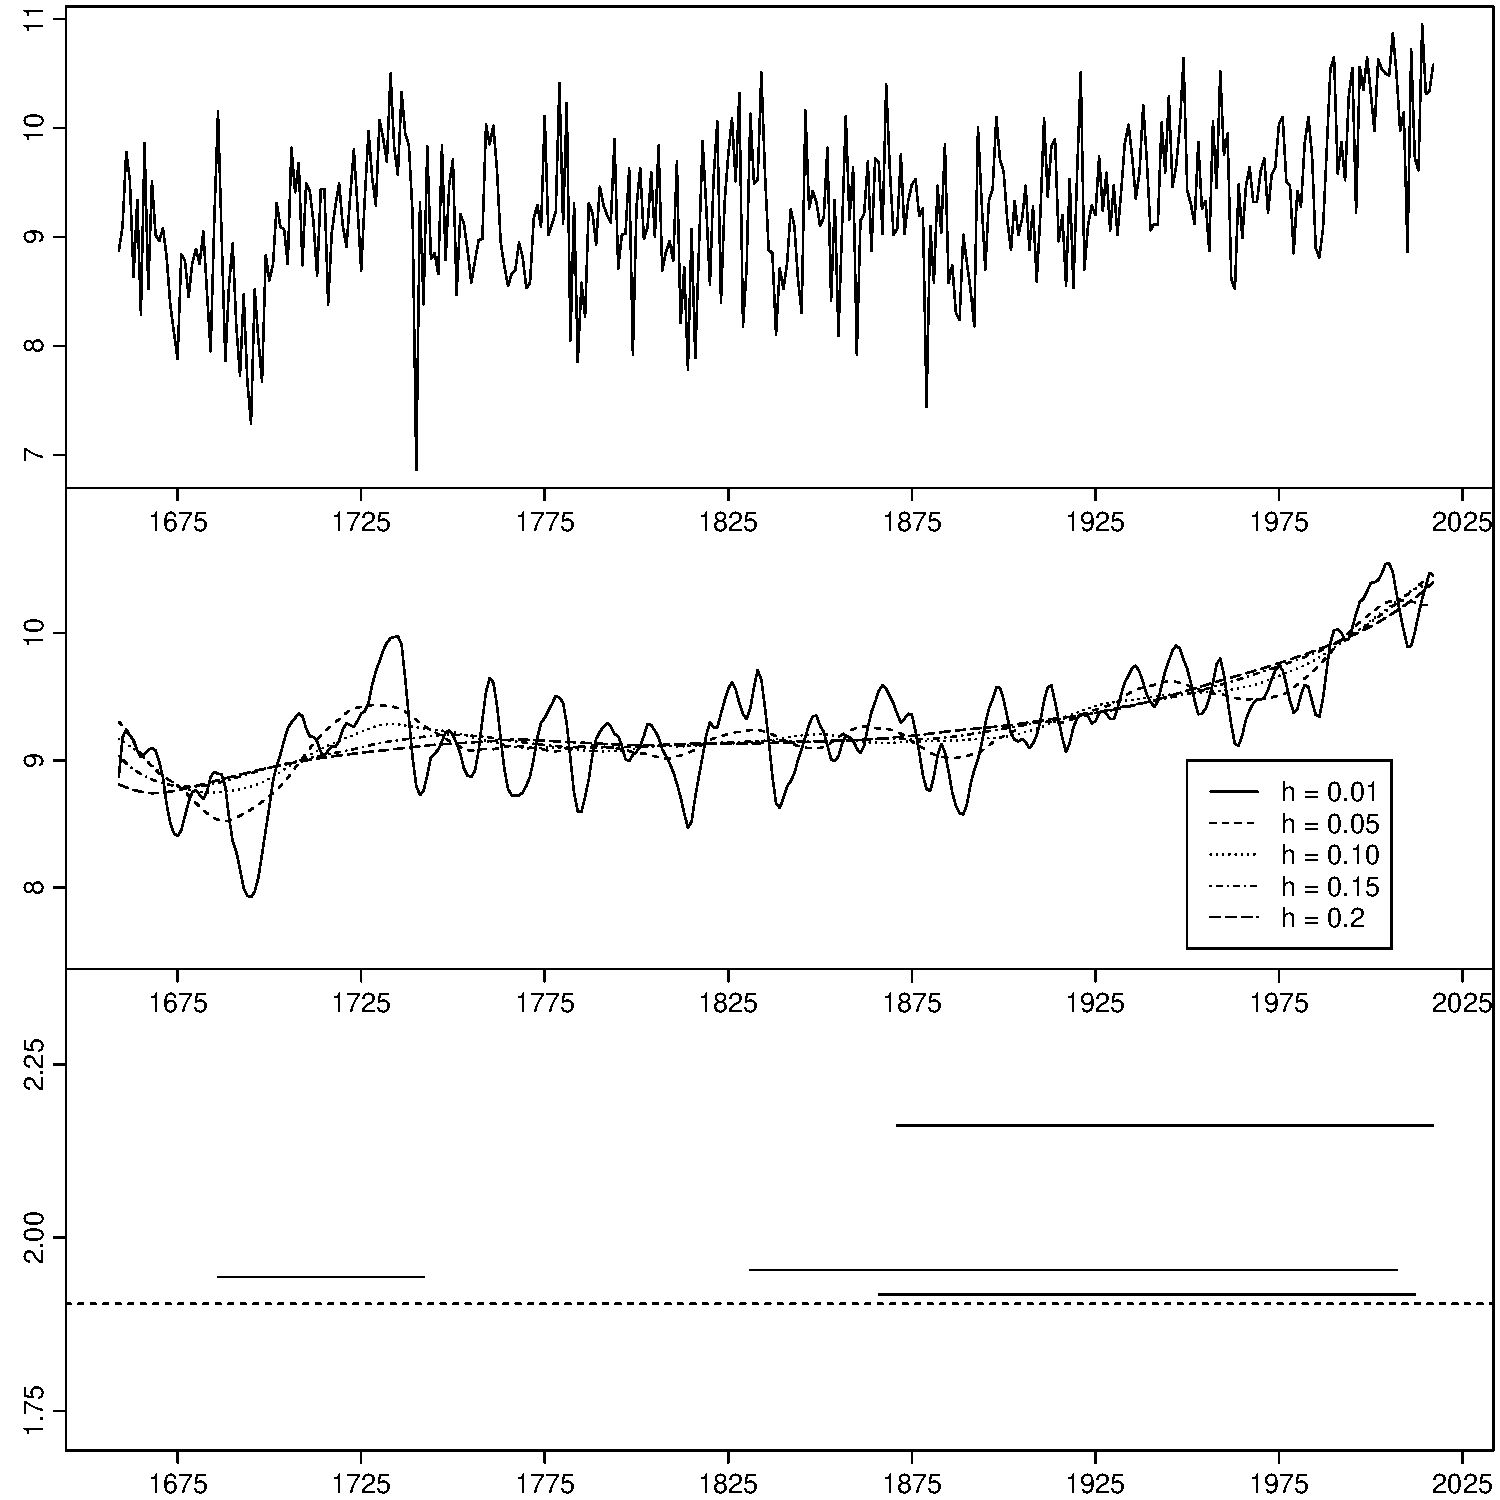
\includegraphics[height=0.85\textheight]{threegraphics_testing_constant_method_ll.pdf}
    %\caption{Summary of the application results for testing shape}
    \label{figure:shape_results}
  \end{figure}
\end{frame}

\begin{frame}{Simulation results of the multiscale test for constant trend function}
\scriptsize{\begin{table}[t]
\begin{center}
\caption{Size of the multiscale test.}
\label{tab:size_shape}
% latex table generated in R 3.4.3 by xtable 1.8-2 package
% 
\begin{tabular}{cccc}
  \hline
  & \multicolumn{3}{c}{nominal size $\alpha$} \\
 $T$ & 0.01 & 0.05 & 0.1 \\
 \hline
250 & 0.004 & 0.022 & 0.082 \\ 
  350 & 0.007 & 0.031 & 0.067 \\ 
  500 & 0.011 & 0.056 & 0.086 \\ 
  1000 & 0.011 & 0.060 & 0.098 \\ 
   \hline
\end{tabular}

\end{center}
\end{table}}
\begin{center}
\normalsize{Power of the multiscale test for different slope parameters $\beta$.}
\end{center}
\vspace{-5mm}
\scriptsize{\begin{columns}
\begin{column}[b]{0.33\textwidth}
\begin{table}[t]
\centering
\caption{$\beta = 1.25$}\label{tab:power_050_ll_shape}
% latex table generated in R 3.4.3 by xtable 1.8-2 package
% 
\begin{tabular}{cccc}
  \hline
  & \multicolumn{3}{c}{nominal size $\alpha$} \\
 $T$ & 0.01 & 0.05 & 0.1 \\
 \hline
250 & 0.107 & 0.223 & 0.358 \\ 
  350 & 0.216 & 0.374 & 0.500 \\ 
  500 & 0.280 & 0.554 & 0.678 \\ 
  1000 & 0.756 & 0.910 & 0.935 \\ 
   \hline
\end{tabular}

\end{table}
\end{column}
\begin{column}[b]{0.33\textwidth}
\begin{table}[t]
\centering
\caption{$\beta = 1.875$}\label{tab:power_075_ll_shape}
% latex table generated in R 3.4.3 by xtable 1.8-2 package
% 
\begin{tabular}{cccc}
  \hline
  & \multicolumn{3}{c}{nominal size $\alpha$} \\
 $T$ & 0.01 & 0.05 & 0.1 \\
 \hline
250 & 0.365 & 0.582 & 0.709 \\ 
  350 & 0.644 & 0.779 & 0.845 \\ 
  500 & 0.784 & 0.942 & 0.976 \\ 
  1000 & 0.997 & 1.000 & 1.000 \\ 
   \hline
\end{tabular}

\end{table}
\end{column}
\begin{column}[b]{0.33\textwidth}
\begin{table}[t]
\centering
\caption{$\beta = 2.5$}\label{tab:power_100_ll_shape}
% latex table generated in R 3.4.3 by xtable 1.8-2 package
% 
\begin{tabular}{cccc}
  \hline
  & \multicolumn{3}{c}{nominal size $\alpha$} \\
 $T$ & 0.01 & 0.05 & 0.1 \\
 \hline
250 & 0.717 & 0.875 & 0.928 \\ 
  350 & 0.933 & 0.977 & 0.989 \\ 
  500 & 0.989 & 0.999 & 1.000 \\ 
  1000 & 1.000 & 1.000 & 1.000 \\ 
   \hline
\end{tabular}

\end{table}
\end{column}
\end{columns}}
\end{frame}


\section{Conclusion}
\begin{frame}{Conclusion}
We developed multiscale methods to test qualitative hypothese about nonparametric time trends:
\begin{itemize}
\item whether the trend is present at all;
\item whether the trend function is constant;
\item in which time regions there is an upward/downward movement in the trend.
\end{itemize}
We derived asymptotic theory for the proposed tests.

As an application of our method, we analyzed the behavior of the yeraly mean temperature in Central England from 1659 to 2017.
\end{frame}


\begin{frame}[standout]
  Thank you!
\end{frame}




\appendix





\begin{frame}
\thispagestyle{empty}
\begin{center}
\Large{\textbf{Testing for equality of the time trends}}
\end{center}
\end{frame}

\begin{frame}{Model}
We observe $n$ time series $\mathcal{Y}_i = \{Y_{it}: 1 \le t \le T \}$ of length $T$ for $1 \le i \le n$
\begin{equation*}\label{model2}
Y_{it} = m_i \Big( \frac{t}{T} \Big) + \alpha_i +\varepsilon_{it} 
\end{equation*}\pause
\vspace{-3mm}
where
\begin{itemize}
\item $m_i$ is an unknown trend function on $[0,1]$, that are Lipschitz continuous and normalized such that $\int_0^1 m_i(u)du = 0$;
\item $\alpha_i$ is an intercept term;
\item $\mathcal{E}_i = \{ \varepsilon_{it}: 1 \le t \le T \}$ is a zero-mean stationary error process;
\item $\mathcal{E}_i$ are independent across $i$.
\end{itemize}
\end{frame}

\begin{frame}{Model}
Not observed variables
\begin{equation*}\label{model2}
Y^o_{it} = Y_{it} - \alpha_i = m_i \Big( \frac{t}{T} \Big) +\varepsilon_{it} 
\end{equation*}
can be approximated by 
\begin{equation*}\label{model2}
\widehat{Y}_{it} = Y_{it} - \widehat{\alpha}_i = Y_{it} - \frac{1}{T}\sum_{i=1}^T Y_{it}.
\end{equation*}
By construction 
\begin{equation*}\label{model2}
Y^o_{it} - \widehat{Y}_{it} = \widehat{\alpha}_i - \alpha_i = \frac{1}{T}\sum_{i=1}^T \varepsilon_{it} + \frac{1}{T}\sum_{i=1}^T m_i(t/T) = O_P(T^{-1/2}).
\end{equation*}
\end{frame}

\begin{frame}{Test Statistic}
For a given location $u \in [0,1]$, bandwidth $h$ and a pair of time series $i$ and $j$ we construct the kernel averages
\begin{equation*}
\widehat{\psi}_{ij,T}(u,h) = \sum\limits_{t=1}^T w_{t,T}(u,h) {\color<2->{mLightBrown}(\widehat{Y}_{it} - \widehat{Y}_{jt})}, 
\end{equation*}\pause
\vspace{-3mm}
where 
\begin{align*}
w_{t,T}(u,h) &= \frac{\Lambda_{t,T}(u,h)}{ \{\sum\nolimits_{t=1}^T \Lambda_{t,T}^2(u,h)\}^{1/2} } ,\\
\Lambda_{t,T}(u,h) &= K\Big(\frac{t/T-u}{h}\Big) \Big[ S_{T,2}(u,h) - S_{T,1}(u,h) \Big(\frac{t/T-u}{h}\Big) \Big], \\
S_{T,\ell}(u,h) &= \frac{1}{Th} \sum\nolimits_{t=1}^T K\Big(\frac{t/T-u}{h}\Big) \Big(\frac{t/T-u}{h}\Big)^\ell
\end{align*}
for $\ell = 0,1,2$ and $K$ is a kernel function.
\end{frame}

\begin{frame}{Test Statistic}
Our multiscale statistic is defined as follows
\begin{align*}
\color<2>{mLightBrown}\widehat{\Psi}_{n,T} & \color<2>{mLightBrown}=\max_{1\le i < j \le n}\widehat{\Psi}_{ij,T}, \\
\widehat{\Psi}_{ij,T} &= \max_{(u,h) \in \mathcal{G}_T} \Big\{ \Big|\frac{\widehat{\psi}_{ij,T}(u,h)}{{\color<2>{mLightBrown}(\widehat{\sigma}_i^2 + \widehat{\sigma}_j^2)^{1/2}}}\Big| - \lambda(h) \Big\}, 
\end{align*} 
where 
\begin{itemize}
\item $\lambda(h) = \sqrt{2 \log \{ 1/(2h) \}}$ is an additive correction term;
\item $\mathcal{G}_T$ is the set of points $(u,h)$ that are taken into consideration;
\item $\widehat{\sigma}^2_i$ is an appropriate estimator of the long-run variance $\sigma^2_i$.
\end{itemize}
\end{frame}

\begin{frame}{Test procedure}
Testing problem:
\vspace{-3mm}
\begin{align*}
H_0: \quad m_1 = m_2 = \ldots = m_n
\end{align*} \pause
\vspace{-2mm}
Gaussian version of the test statistic:
\begin{align*}
\color<3->{mLightBrown}\Phi_{n, T} &\color<3->{mLightBrown}= \max_{1 \le i < j \le n} \Phi_{ij, T},\\
\Phi_{ij,T} &= \max_{(u,h) \in \mathcal{G}_T} \Big\{ \Big|\frac{\phi_{ij,T}(u,h)}{{\color<3->{mLightBrown}(\widehat{\sigma}_i^2 + \widehat{\sigma}_j^2)^{1/2}}}\Big| - \lambda(h) \Big\},
\end{align*} 
\vspace{-3mm}
where
\begin{align*}
\phi_{ij,T}(u,h) = \sum\nolimits_{t=1}^T w_{t,T}(u,h) \,\Big\{ {\color<3->{mLightBrown}\widehat{\sigma}_i \Big(Z_{it} - \frac{1}{T}\sum_{t=1}^T Z_{it} \Big) - \widehat{\sigma}_j \Big(Z_{jt} - \frac{1}{T}\sum_{t=1}^T Z_{jt}\Big)} \Big\};
\end{align*}
$Z_t$ are independent standard normal random variables;

$q_{n,T}(\alpha)$ is  $(1 - \alpha)$ quantile of $\Phi_{n,T}$.\pause
\begin{block}{Test procedure}
For a given significance level $\alpha \in (0,1)$, we reject $H_0$ if $\widehat{\Psi}_{n,T} > q_{n,T}(\alpha)$.
\end{block}
\end{frame}


\begin{frame}{Theoretical properties}
\begin{prop}\label{prop-equality-1}
Supose that $\mathcal{E}_i$ are independent across $i$ and satisfy $\mathcal{C}1- \mathcal{C}2$ for each $i$. Under our remaining assumptions and under $H_0: m_1 = m_2 =\ldots = m_n$ it holds that 
\vspace{-3mm}
\begin{align*}
\Prob \big( \widehat{\Psi}_{n, T} \le q_{n,T}(\alpha) \big) = (1 - \alpha) + o(1).
\end{align*}
\end{prop}\pause

\begin{prop}\label{prop-equality-2}
Let the conditions of previous proposition be satisfied. Under local alternatives we have
\vspace{-3mm}
\begin{align*}
\Prob \big( \widehat{\Psi}_{n,T} \le q_{n,T}(\alpha) \big) = o(1).
\end{align*}
\end{prop}
\end{frame}

\begin{frame}{Clustering, group structure}
\begin{itemize}
\item The null hypothesis $H_0: m_1 = m_2 = \ldots = m_n$ is violated.
\item There exist sets or groups of time series $G_1,\ldots,G_N$ with $N \le n$ and $\{1,\ldots,n\} = \mathbin{\dot{\bigcup}}_{\ell=1}^{N} G_\ell$ such that for each $1 \le \ell \le N$ we have $m_i = g_\ell \quad \text{for all } i \in G_\ell$, where $g_\ell$ are group-specific trend functions.
\item For any $\ell \ne \ell^\prime$, the trends $g_{\ell,T}$ and $g_{\ell^\prime,T}$ differ in the following sense: There exists $(u,h) \in \mathcal{G}_T$ with $[u-h,u+h] \subseteq [0,1]$ such that $g_{\ell,T}(w) - g_{\ell^\prime,T}(w) \ge c_T \sqrt{\log T/(Th)}$ for all $w \in [u-h,u+h]$ or $g_{\ell^\prime,T}(w) - g_{\ell,T}(w) \ge c_T \sqrt{\log T/(Th)}$ for all $w \in [u-h,u+h]$, where $0 < c_T \rightarrow \infty$.
\end{itemize}
\end{frame}

\begin{frame}{Clustering, algorithm}
Dissimilarity measure between two sets of time series $S$ and $S^{\prime}$:
\begin{equation*}\label{dissimilarity}
\widehat{\Delta}(S,S^\prime) = \max_{\substack{i \in S, \\ j \in S^\prime}} \widehat{\Psi}_{ij,T}. 
\end{equation*}
\begin{center}
\textbf{Clustering algorithm}
\end{center}

\textit{Step $0$ (Initialization):} Let $\widehat{G}_i^{[0]} = \{ i \}$ denote the $i$-th singleton cluster for $1 \le i \le n$ and define $\{\widehat{G}_1^{[0]},\ldots,\widehat{G}_n^{[0]} \}$ to be the initial partition of time series into clusters. 

\noindent \textit{Step $r$ (Iteration):} Let $\widehat{G}_1^{[r-1]},\ldots,\widehat{G}_{n-(r-1)}^{[r-1]}$ be the $n-(r-1)$ clusters from the previous step. Determine the pair of clusters $\widehat{G}_{\ell}^{[r-1]}$ and $\widehat{G}_{{\ell}^\prime}^{[r-1]}$ for which 
\begin{align*}
\widehat{\Delta}(\widehat{G}_{\ell}^{[r-1]},\widehat{G}_{{\ell}^\prime}^{[r-1]}) = \min_{1 \le k < k^\prime \le n-(r-1)} \widehat{\Delta}(\widehat{G}_{k}^{[r-1]},\widehat{G}_{k^\prime}^{[r-1]})
\end{align*}
and merge them into a new cluster. 
\end{frame}

\begin{frame}{Clustering, theoretical properties}
The estimator of the number of groups is
\begin{align*}
\widehat{N} = \min \Big\{ r = 1,2,\ldots \Big| \max_{1 \le \ell \le r} \widehat{\Delta} \big( \widehat{G}_\ell^{[n-r]} \big) \le q_{n,T}(\alpha) \Big\}.
\end{align*}\pause
\begin{prop}\label{prop-clustering-1}
Let the conditions of previous propositions be satisfied. Then 
\begin{align*}
\Prob \Big( \big\{ \widehat{G}_1,\ldots,\widehat{G}_{\widehat{N}} \big\} = \{ G_1,\ldots,G_N \} \Big) \ge (1-\alpha) + o(1)
\end{align*}
and 
\begin{align*}
\Prob \big( \widehat{N} = N \big) \ge (1-\alpha) + o(1).
\end{align*}
\end{prop}
\end{frame}
\begin{frame}{Testing for equality of different temperature time trends}
  \begin{figure}
    \centering
    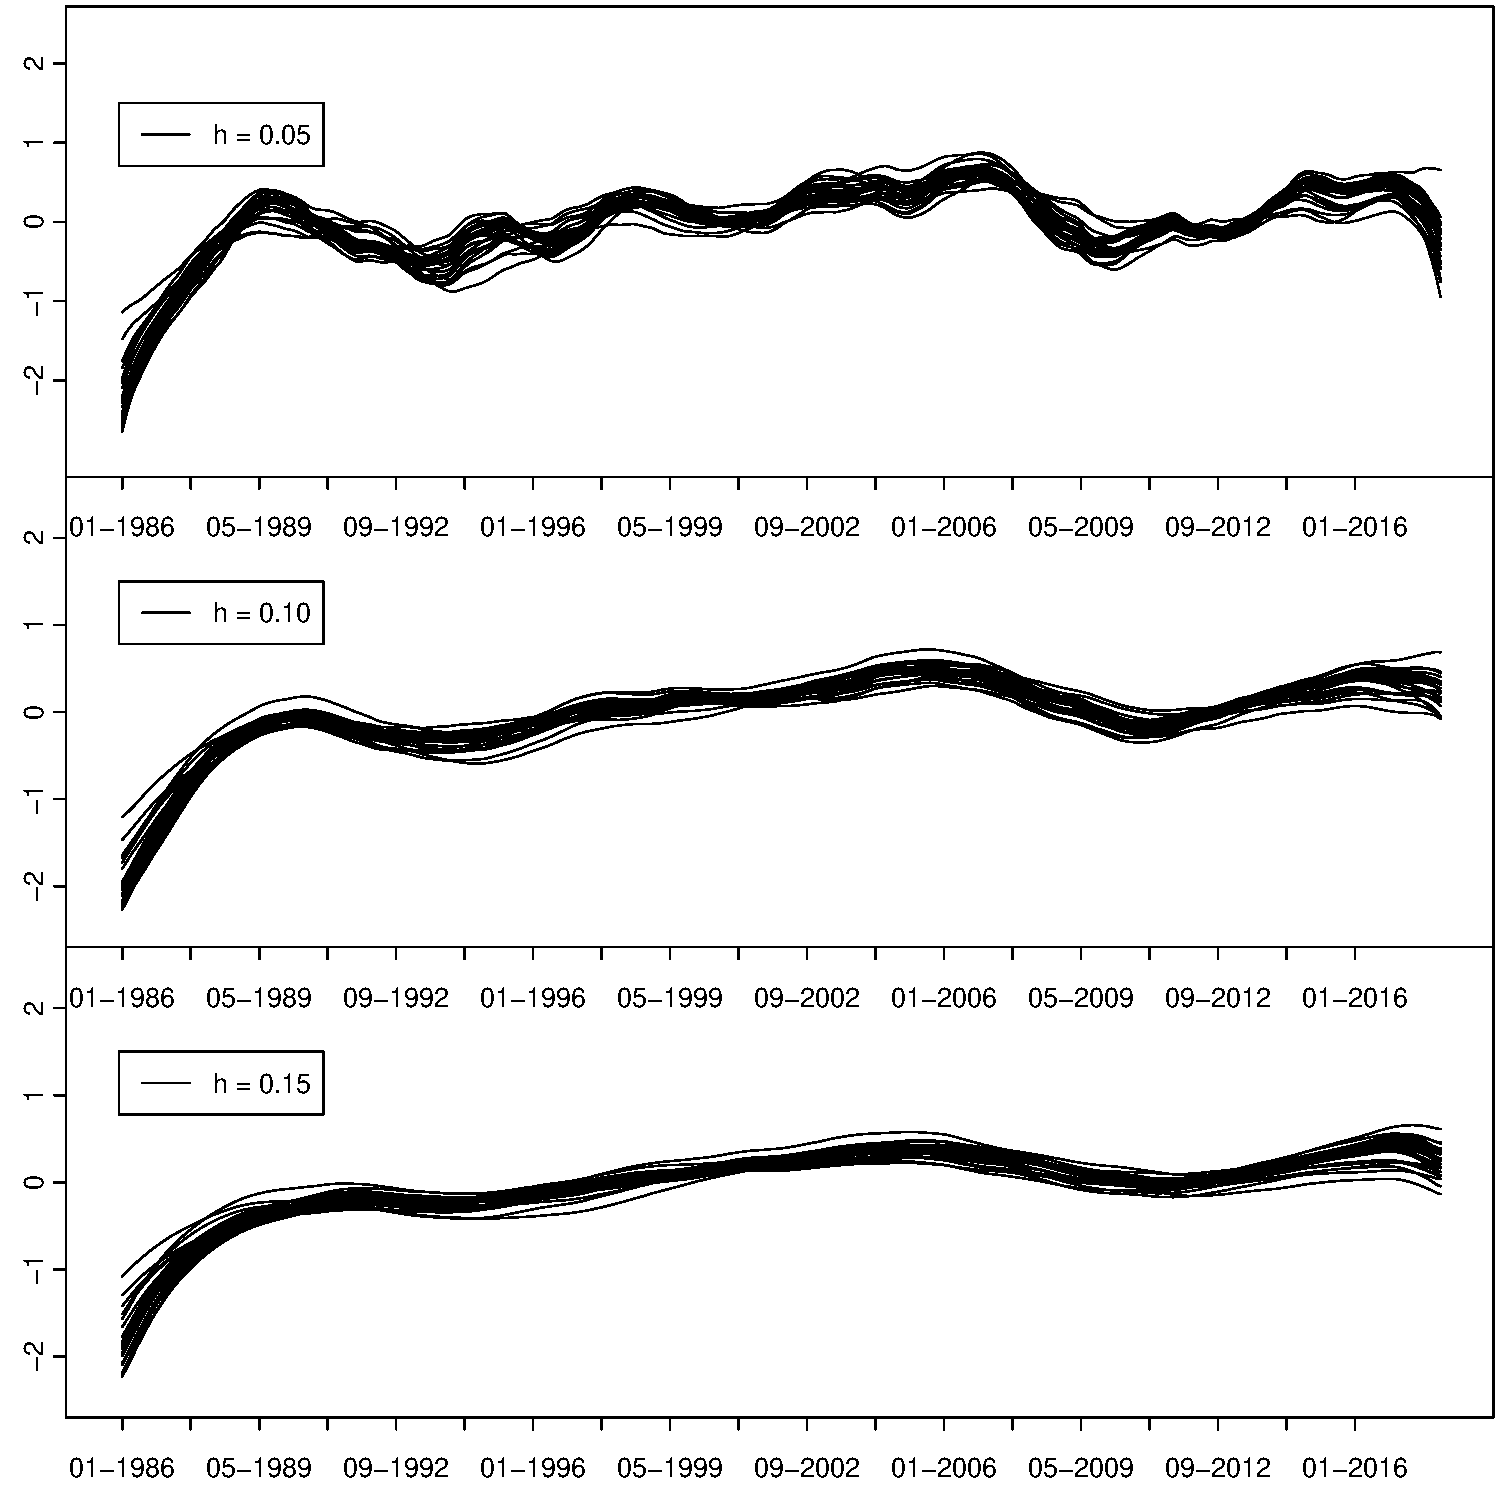
\includegraphics[height=0.85\textheight]{stations_data.pdf}
    %\caption{Local linear kernel estimates of the $n = 25$ time trends}
    \label{figure:station_data}
  \end{figure}
\end{frame}

\begin{frame}[label = frame_lambda]{Idea behind the additive correction}
\onslide<1->{Consider the uncorrected statistic
\begin{align*}
\widehat{\Psi}_{T, \text{uncorrected}} = \max_{(u,h) \in \mathcal{G}_T} \Big|\frac{\widehat{\psi}_T(u,h)}{\widehat{\sigma}}\Big|
\end{align*}
under the null hypothesis $H_0: m = 0$ and under simplifying assumptions:
\begin{itemize}
\item the errors $\varepsilon_i$ are i.i.d. normally distributed;
\item $\widehat{\sigma} = \sigma$;
\item $\mathcal{G}_T = \{(u_k, h_l) | u_k = (2k - 1)h_l \text{ for } 1\le k \le 1/2h_l, 1 \le l \le L\}$.\pause
\end{itemize}}
\only<2>{
\begin{align*}
\widehat{\Psi}_{T, \text{uncorrected}} = \max_{1 \le l \le L} \max_{1\le k \le 1/2h_l} \Big|\frac{\widehat{\psi}_T(u_k,h_l)}{\sigma}\Big|
\end{align*}}
\onslide<3->{\begin{align*}
\widehat{\Psi}_{T, \text{uncorrected}} = \max_{1 \le l \le L} \max_{1\le k \le 1/2h_l} \Big|{\color{mLightBrown}\frac{\widehat{\psi}_T(u_k,h_l)}{\sigma}}\Big|
\end{align*}}
\onslide<4->{$\Rightarrow \quad \max_k \frac{\widehat{\psi}_T(u_k,h_l)}{\sigma} ={\color<5->{mLightBrown}\sqrt{2\log(1/2h_l)}} + o_P(1) \to \infty$ as $h \to 0$ and the stochastic behavior of $\widehat{\Psi}_{T, \text{uncorrected}}$ is dominated by $\frac{\widehat{\psi}_T(u_k,h_l)}{\sigma}$ for small bandwidths $h_l$. \hyperlink{frame_teststatistic}{\beamerbutton{Go back}}}
\end{frame}

\end{document}
